\section{Resultados}
\label{ch:resultados}

\subsection{Estado final}
\label{sec:estado_final}

Al cierre de la Estadía, las 129 alertas de AWS registradas en el diagnóstico inicial se clasificaron por completo entre patrones programados y fallas reales; ese trabajo tomó varios días de revisión continua.

El script de monitoreo de TIBCO Scribe también evolucionó respecto a la primera versión descrita en Metodología. En la versión final, la regla del estado de error fatal —que en un inicio se seguía revisando de forma manual— quedó automatizada: el script revisa el historial completo de cada solución, reporta cada ejecución en error fatal de forma individual sin repetir el mismo evento dos veces, y evita alertar sobre caídas que ya existían antes de que el script arrancara, para no saturar de avisos viejos. También se agregó la posibilidad de silenciar temporalmente, mediante un comando enviado al bot de Telegram, las alertas de una solución específica cuando el equipo ya tenía conocimiento de una falla en curso.

\subsection{Comparativo antes/después}
\label{sec:comparativo}

Antes de contar con el script, revisar a mano el estado de las soluciones de TIBCO Scribe tomaba entre 3 y 4 minutos por cada institución educativa: había que seleccionar cada solución en el menú, aplicar el filtro y esperar el resultado de la consulta, unas 16 veces por cliente. La ronda completa de las dos instituciones, es decir las 32 soluciones, tomaba entre 6 y 7 minutos, y se repetía cada 30 minutos durante toda la jornada. Con el script, esa misma ronda se hace sola cada 4 minutos y no ocupa el tiempo de nadie: el equipo únicamente atiende las notificaciones que el bot envía cuando encuentra una falla real.

\subsection{Evidencia fotográfica}
\label{sec:evidencia_fotografica}

\begin{figure}[h]
    \centering
    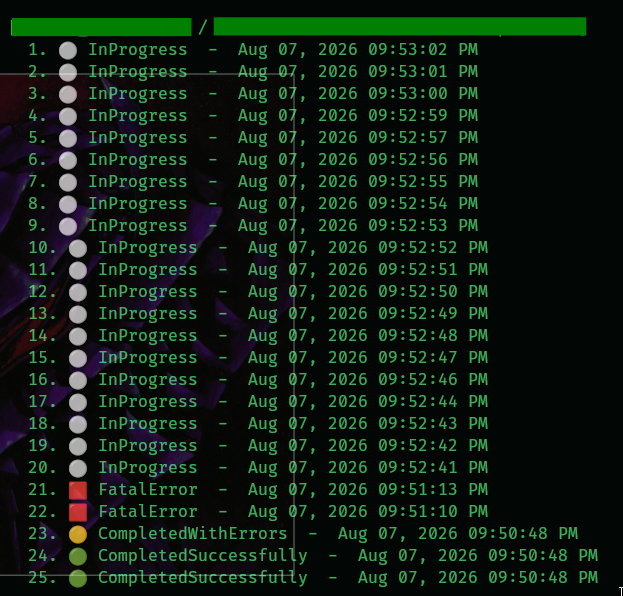
\includegraphics[width=0.8\textwidth]{img/figura_bot_estados.png}
    \caption{Los cuatro estados detectados por el bot de monitoreo de TIBCO Scribe.}
    \label{fig:bot_estados}
\end{figure}

\begin{figure}[h]
    \centering
    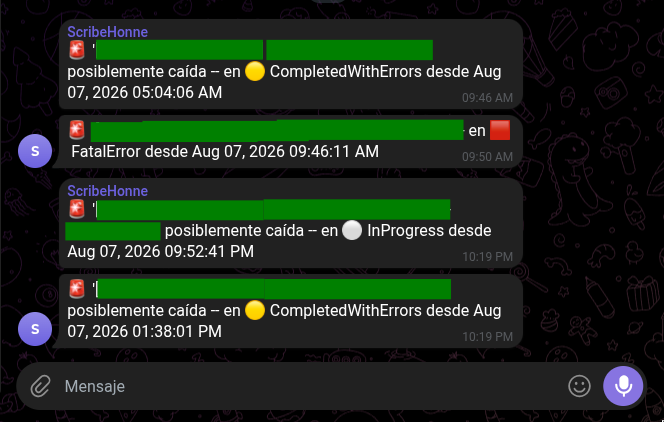
\includegraphics[width=0.8\textwidth]{img/figura_telegram_aviso.png}
    \caption{Avisos reales enviados por el bot al grupo de Telegram del equipo.}
    \label{fig:telegram_aviso}
\end{figure}

\subsection{Análisis de los resultados}
\label{sec:analisis_resultados}

El objetivo de automatizar el monitoreo de TIBCO Scribe se cumplió por completo: la versión final del script cubre incluso la regla del estado de error fatal, que en un inicio se seguía revisando de forma manual. Al dejar de hacerse cada 30 minutos de forma manual, el equipo pudo destinar ese tiempo a atender incidentes reales y otras tareas de monitoreo en lugar de revisiones repetitivas.

En el caso de AWS y Google Cloud Platform, el objetivo de verificar y reportar alertas también se cumplió, pero de forma manual en ambos casos; a diferencia de TIBCO Scribe, no se llegó a desarrollar una automatización similar para ellas, principalmente porque el tiempo de la Estadía se concentró en la herramienta que representaba la carga de trabajo más repetitiva. Para ServiceNow, esa automatización sí llegó a existir, pero fue obra de un compañero del equipo, no de este trabajo. Esa automatización pendiente para AWS y GCP queda como una oportunidad de mejora a futuro.
